In this chapter we present the JS-QL tool. The tool offers the possibility for developers to write application-specific queries to check for certain program properties. More specifically, the tool offers a solution to developers for testing their applications for vulnerabilities by writing and enforcing security policies for these applications. We use the JIPDA abstract state graph as the program's representation, and we check check all queries against the graph. The tool consists of three main parts: 
\begin{enumerate}
\item \textit{The JS-QL query language}: Short for \textbf{J}ava\textbf{S}cript \textbf{Q}uery \textbf{L}anguage. It is a domain-specific language in which users can express different kinds of security vulnerabilities. An overview of the language is given in section \ref{sec:Syntax}.
\item \textit{The matching engine}: The engine is the core of the tool. It matches user-defined queries against states in a JIPDA abstract state graph, capturing and unifying relevant program properties.
\item \textit{The graphical user interface}: The user interface provides the infrastructure for the developer to interact with the tool. It contains a section where users can specify the input program and a security policy, a graphical component representing the abstract state graph corresponding to the input program and a visual and textual representation of the query results. The textual representation allows developers to inspect the captured variables, a useful feature when these variables are compound data structures. The user interface is depicted in figure \ref{fig:UI}.
\end{enumerate}

The abstract state graph obtained from the JIPDA analysis is a suitable starting point to inspect a program for certain characteristics and security vulnerabilities. In chapter \ref{ch:Overview} we motivated our choice to design an internal DSL to query for specific (sequences of) states in this graph, with the aim to discover program patterns that might lead to violations of user-defined security policies. The language constructs are designed to facilitate the specification of patterns that must be detected. 

The remainder of this chapter presents all facets of the JS-QL language: Section \ref{sec:Syntax} discusses all constructs of the language and gives an in-depth explanation on how to correctly use them. As different security vulnerabilities require different traversals of the state graph, more than one type of query is needed. We discuss the difference between several query types in section \ref{sec:TypesOfQueries}. In order to have an effective specification language, we must enable the user to create compound queries out of the available language constructs. Section \ref{sec:DefiningPolicies} shows how this can be done in the tool.

\section{The JS-QL query language}
\label{sec:Syntax}
 In this section we discuss the syntax and semantics of the JS-QL language. The examples in this section are kept simple to demonstrate how each construct works. For more advanced queries and security vulnerabilities, we refer to chapter \ref{ch:Evaluation}.

%Entry point
\subsection{The entry point}
JS-QL is an internal DSL, meaning that it is embedded in a host language, and that the host language has to provide an entry point from where we can start using JS-QL. In our approach the \texttt{G} object, short for \textbf{G}raph, is the entry point. This implies that all query patterns in JS-QL will start from this object. Example \ref{ex:G} shows how \texttt{G} can be used.

\begin{exmp}
\label{ex:G}
Listing \ref{lst:entryPoint} shows a query where the first state of the graph is matched, starting with entry point \texttt{G}.

\begin{lstlisting}[label={lst:entryPoint},language=JSQL,caption=Matching the first state starting from entry point \texttt{G},mathescape=true]  % float=t?

//Match the first state of the graph
G.state()
\end{lstlisting}
\end{exmp}

\subsection{State}
The \texttt{state} construct is the single most basic element of the language. It matches any state in the graph, but does not provide other information. Nevertheless is it the most important building block of the language, as it can be used to construct higher-level queries and predicates. 

\subsubsection*{Keywords}
States can be made more precise and expressive by parametrizing them with \textit{state keywords}. We will first give a short overview of what information is available in which states. To get a more detailed explanation on what each piece of information represents, we refer to the section about flow graphs (\ref{sec:FlowGraphs}). Table \ref{tab:InfoPerState} indicates what information is available in which type of state. The table also shows which keyword is used to represent the information contained in the states.

\begin{table}[!h]
\centering
\caption*{
  \centering
  	\begin{tabular}{| l | c |}
  	\hline
  	\multicolumn{2}{ |c| }{Legend} \\
  	\hline
  	Evaluation state & $E$  \\
  	Continuation state & $K$  \\
  	Return state & $R_t$  \\
  	Result state & $R_s$  \\
  	All states & $A$  \\
  	\hline
  	\end{tabular}
  	%$E$ = EvalState, $K$ = KontState, $R_t$ = ReturnState, $R_s$ = ResultState, $A$ = All states
  }
  \begin{tabular}{| l | l | c |}
  \hline
  State property & Available in states & Keyword\\
  \hline
  Node & $E$ & node\\
  Meta continuation & $A$ & kont\\
  Local continuation & $A$ & lkont\\
  Binding environment & $E$ & benv\\
  Store & $A$ & store\\
  Value & $K$ $R_t$ $R_s$ & value\\ \hline \hline
  Identifier & $A$ & \_id\\
  Successors & $A$ & \_successors \\
  \hline

  \end{tabular}
  
  \caption{Information in the states of the abstract state graph}
  \label{tab:InfoPerState}
\end{table}

To improve readability, JS-QL provides four extra constructs that are semantically almost equivalent to the regular \texttt{state} construct. \texttt{evalState}, \texttt{kontState}, \texttt{returnState} and \texttt{resultState} are included in the language to match only those specific kinds of states.
Note that the tool also supports the usage of the identifier and successors of a state, but it is very uncommon to use them, as they are semantically irrelevant to queries. An identifier is a unique value, used to distinguish different states. The identifier of a state would only be relevant when a query is matched in that exact state. When this is the case, the state gets marked in the visual graph representation and all query information is then contained in that state. Successors also contain few additional information, as all direct successors of a state are already made explicit in the state graph. 

\subsubsection*{Parametrizing a state}
 Variables in JS-QL are strings starting with a \texttt{?}. The fact that we use strings comes from the embedded nature of our language: If we were to specify variables as literals, the host language would complain that it does not recognize the literal. This is illustrated in example \ref{ex:Parametrizing}.

\begin{exmp}
\label{ex:Parametrizing}
The query on line 2 of listing \ref{lst:stringVariables} depicts a JS-QL query that captures the \textit{type} property of the node in variable \texttt{'?nType'}. If we omit the quotes around the variable, the syntax would not be recognized by the host language, as seen on line 4.

\begin{lstlisting}[label={lst:stringVariables},language=JSQL,caption=Defining variables in JS-QL,mathescape=true]  % float=t?

//Capture the 'type' property of the node in variable '?nType'
G.state({ node : { type: '?nType' }})
//Exception: ?nType is not recognized by the host language
G.state({ node : { type: ?nType }}) 
\end{lstlisting}

\end{exmp}

As the example indicates, JS-QL deconstructs state properties as nested key-value pairs. In this way, each part of information can be captured in a variable. The key indicates the property to be matched whereas the value can be one of three things:
\begin{enumerate}
\item A \textit{variable}. When placing a variable as the value in a key-value pair in JS-QL, that variable gets bound to the key's corresponding value in the JIPDA state. The \texttt{?nType} variable in the example above gets bound to the value of \texttt{type}, which in this case corresponds with the type of the AST \texttt{node} for the currently matched state.
\item A \textit{nested map} which further deconstructs the current property. The example above does this by further deconstructing the \texttt{node} property of a state (which represents the corresponding AST node) in order to reach the \texttt{type} of that node and store it in a variable. This is primarily used to match specific AST nodes.
\item A \textit{literal}. Literals are mostly used to filter the states to be matched. When applying this to the example above, the '?nType' variable could be replaced by the literal 'ExpressionStatement' for example. Note that the question mark (\texttt{?}) is omitted. The resulting query would then only match a state having the \texttt{type} of its corresponding AST \texttt{node} equal to 'ExpressionStatement'.
\end{enumerate}


\noindent States can thus be parametrized by matching the keywords displayed in table \ref{tab:InfoPerState} as keys with values that can be variables, literals or nested maps. Because queries matching single-state patterns are not yet security policies, JS-QL enables users to specify sequences of states as a query. When checking the state graph against this query, all states in the query pattern need to be matched one after another. When a state in the query pattern is encountered that does not match the current state in the state graph, the matching process is aborted for the current path that is investigated in the state graph. Consider the query in listing \ref{lst:Unification}:

\begin{lstlisting}[label={lst:Unification},language=JSQL,caption=Unification in JS-QL,mathescape=true]  % float=t?

G.state({ node : { type: '?t' }})
 .state({ node : { type: '?t' }})
\end{lstlisting}

\noindent Variable \texttt{?t} occurs twice in the query. This can be done on purpose to achieve \textit{unification}. Unification means that two variables with the same name have to contain the same value. After executing the first line, the first state in the graph is matched (assuming that it has the \texttt{node} property) and the variable \texttt{?t} is bound to the type of the node. The matching engine then proceeds to the next state in both the query and the state graph. If the next state again has the \texttt{node} property with the same type as already bound to \texttt{?t}, the unification process has succeeded and the whole query will match. If the node type of the next state isn't equal to the value already bound to \texttt{?t}, or if that state doesn't have a \texttt{node} property, there is no match. The results of a successfully matched query will be the set of all possible \textit{substitutions}, together with the identifier of the state where the last element of the query matched. Figure \ref{fig:Unification} gives a simplistic visual representation of this process.

\begin{figure}[!h]
    \centering
      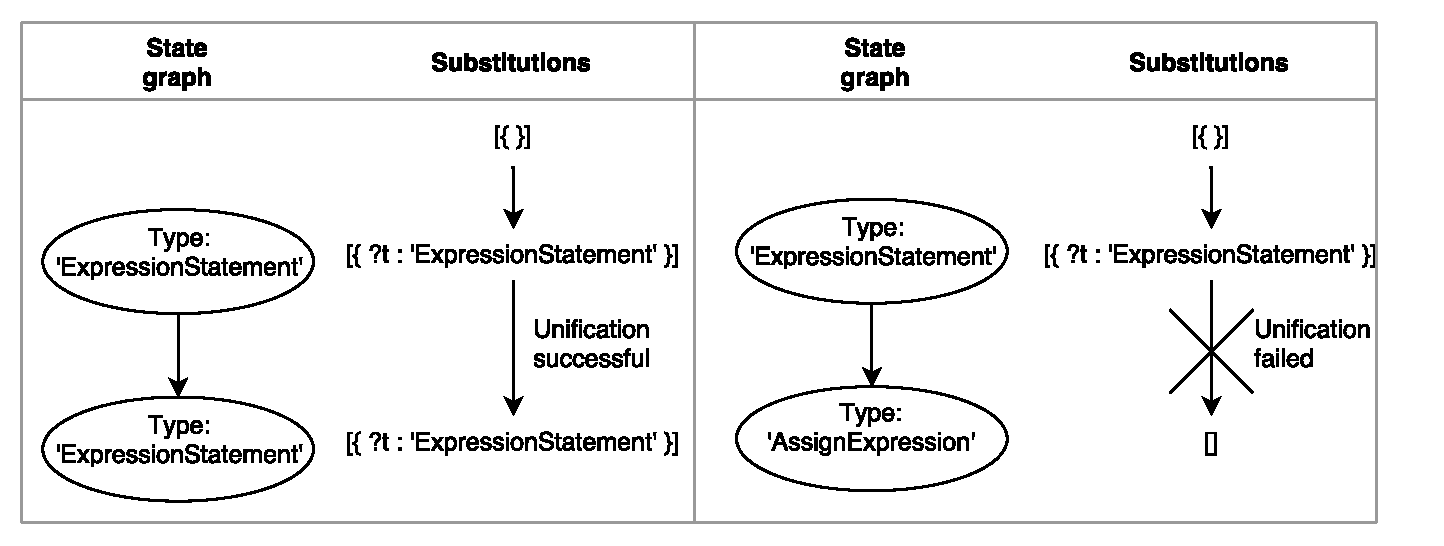
\includegraphics[width=1\textwidth]{images/Unification} 
      \caption{Visual representation of the unification process}
    \label{fig:Unification}
\end{figure}

All queries presented up until now match the state graph from the beginning of the graph only. This behaviour is often undesirable as a developer usually wants to detect a pattern \textit{somewhere} in his code, not necessarily at the beginning. To resolve this, JS-QL combines techniques from regular expressions with a special built-in construct, the \textit{wildcard}.


\subsection{Wildcard}

A wildcard can be described as a placeholder for 'things of which the value can be anything'. A \texttt{wildcard} serves the sole purpose of matching any state it gets compared with. In other words, another name for this construct would be \texttt{skip}, as it skips a state in both the query (the \texttt{wildcard} state itself) and the abstract state graph (the state the wildcard gets matched with). When talking about states in a query pattern, both \texttt{state} and \texttt{wildcard} match this definition. \texttt{wildcard}s act just like regular \texttt{state}s in a query, meaning that they only match \textit{1} state in the state graph. 

\subsubsection*{Skipping multiple states}

It is very unlikely that a developer knows exactly after how many states a violation would occur, so simply enumerating wildcards followed by the state to be matched would typically be a very tiresome effort. We therefore need to be able to specify that we wish to skip \textit{zero or more} states before matching the following state in the query pattern. 

This is where the power of regular expressions is useful. Just like regular expressions, JS-QL supports the use of both the Kleene star (\texttt{star}) and the Kleene plus (\texttt{plus}) operators. In our language, the \texttt{star} and \texttt{plus} constructs are both placed \textit{after} the state(s) they are applied to. Placing \texttt{star} behind a state indicates that that statencan occur \textit{zero or more} times at the current position in the state graph. The semantics of \texttt{plus} are very similar, except for the fact that the state has to occur at least once. 

Just like with regular expressions, pieces of a pattern can be surrounded by braces. Left and right braces in JS-QL are denoted by \texttt{lBrace} and \texttt{rBrace} respectively. The default behavior of both the Kleene star and Kleene plus operators is to apply them to the state that occurs right before it. If any Kleene operator has to be applied to multiple states, these states have to be wrapped in braces in JS-QL. The different uses of the Kleene operators are depicted in example \ref{ex:Kleene}

\begin{exmp}
\label{ex:Kleene}
 Listing \ref{lst:KleeneOperations} shows the differences in using the Kleene operators with and without braces. Lines 1 and 2 are semantically equivalent, as the braces on line 2 only contain 1 state, a \texttt{wildcard} in this case. Lines 3 and 4 on the other hand are semantically different. The query on line 3 matches all but the first states in the state graph, whereas the query on line 4 matches every other state in the graph, starting from the second state. The combinations of \texttt{wildcard().star()} and \texttt{wildcard().plus()} are so commonly used in JS-QL, that a special construct is created for each of them: \texttt{skipZeroOrMore()} and \texttt{skipOneOrMore()} respectively.

\begin{lstlisting}[label={lst:KleeneOperations},language=JSQL,caption=Kleene operations differences,mathescape=true]  % float=t?

G.wildcard().star() // Equal to G.skipZeroOrMore()
G.lBrace().wildcard().rBrace().star()
G.wildcard().state().plus()
G.lBrace().wildcard().state().rBrace().plus()
\end{lstlisting}
\end{exmp}

\subsection{Disjunction}

Sometimes when writing a query, more than one state qualifies as a match. JS-QL provides the \texttt{or} language construct, which enables users to specify that 1 state in the state graph can be matched by multiple states in the query pattern. Consider a simple language in which we want to detect all uses of a variable \texttt{v} in binary arithmetic expressions. When using a variable in a binary arithmetic expression, the variable can be on either side of the operator. A naive solution to query for all uses of \texttt{v} would be to first launch a query that finds all occurences of \texttt{v} on the left-hand side, followed by a query that detects all occurences on the right-hand side. If we then were to match all occurrences of \texttt{v} on the left- and right-hand side of arithmetic expressions, we could write a query as in listing \ref{lst:disjunction}.

\begin{exmp}
\label{ex:Disjunction}
\begin{lstlisting}[label={lst:disjunction},language=JSQL,caption=The JS-QL disjunction operator,mathescape=true]  % float=t?

G.skipZeroOrMore()
.lBrace()
  //Left-hand side with name 'v'
  .state({node: { type: 'BinaryExpression',
                  left: {name:'v'}}})      
  .or()
  //Right-hand side with name 'v'
  .state({node: { type:  'BinaryExpression',
                  right: {name:'v'}}})
.rBrace()
\end{lstlisting}

This query first skips zero or more states, starting from the beginning of the graph. It then matches a \texttt{state} (\texttt{evalState} would be equally correct) with a \texttt{node} property of type 'BinaryExpression'. Remember that the node property of evaluation states contains the AST information for the current expression. Because of this, the \texttt{left} and \texttt{right} properties of the BinaryExpression are again nodes that can be further deconstructed. The \texttt{or} construct splits the query in two different query paths. One path will try to match the pattern specified before the construct, whereas the other path searches for matches for the pattern specified after the \texttt{or}. The same rules apply w.r.t. braces as for the \texttt{star} and \texttt{plus} operators. For the first path, we deconstruct the left property of the node and match its name with the literal \texttt{v}. This automatically filters out all states for which this condition doesn't hold. What remains is a match for each state for which the condition holds. The same is done for the second path, with the only difference that the name of the right node now has to be equal to \texttt{v}.

\end{exmp}

\subsection{Referring to the current object}

The \texttt{this} JS-QL keyword is an implicit property that is made available for each deconstructable map in the language, representing the entire object by which it is encapsulated. The keyword is designed to allow the user to capture a piece of information in a nested map into a variable, while allowing the user to further deconstruct that map. The use of \texttt{this} is demonstrated in example \ref{ex:This}.

\begin{exmp}
\label{ex:This}
When examining example \ref{ex:Disjunction}, we notice that little relevant information is available as a result of the query. A more detailed result should contain the actual node or even the entire state that was matched, so we could inspect it further. Listing \ref{lst:updatedDisjunction} gives an updated version of the relevant code from the previous example. In this version, the \texttt{?thisNode} variable will be bound to the node of the matched state. Without the \texttt{this} keyword, an object could only be stored in a variable by assigning it directly in the nested map, as seen on line 6. This would prohibit the user from further deconstructing the current object, making the language less expressive.

\begin{lstlisting}[label={lst:updatedDisjunction},language=JSQL,caption=Using the \texttt{this} keyword,mathescape=true]  % float=t?

//...
.state({node: { this: '?thisNode',
                type: 'BinaryExpression',
                left: {name:'v'}}})     
//... 
.state({node: '?node'})
\end{lstlisting}

\end{exmp}

\subsection{Specifying additional properties}
\label{subsec:props}

JS-QL has a built-in keyword \texttt{properties}, which can be used to obtain more information from already bound variables. 
Sometimes it can be useful to capture extra information about already matched variables. Doing so via a separate keyword in the language, exclusively designed for this purpose, has two advantages. First of all, it enhances the readability of queries. Queries with deeply nested maps can quickly become confusing to read and bothersome to modify. Secondly, it opens up for opportunities to make the language even more expressive. Expressing properties can be done in two ways, as described in the following two sections.

\subsubsection*{The prop function}
 \texttt{prop} is a function in JS-QL to which the user can pass which kind of information he wish to obtain and from which variable properties need to be obtained. The first argument of \texttt{prop} is the function that needs to be applied when the matching engine processes the query. The arguments of this function are all other arguments that were passed to \texttt{prop}. Example \ref{ex:Properties} shows how to use the \texttt{prop} function. We have to defer the evaluation of the function passed as a first argument to \texttt{prop} because at compile-time the values of the variables areare not yet known (as no matching has happened). This function, in the example, 'memberOf', can be a user-specified function or a built-in function. As for now, JS-QL only has three build-in functions that work on variables, and all three require that variable to be of type \textit{Array}:


\begin{enumerate}
\item \textit{length}: This function can be used as: \texttt{prop('length', '?arr')}, where \texttt{?arr} is a variable with a value of type \texttt{Array}. The function then returns the length of the array bound to the variable.
\item \textit{at}: This function takes 2 additional arguments: A variable containing an array, and an index \texttt{i}. The resulting value is the \texttt{i}th element of the array.
\item \textit{memberOf}: This function takes a variable containing an array \texttt{arr} as an argument and expands the current substitution set, so that for each element in \texttt{arr} a new substitution set is created with that element appended to it.
\end{enumerate}

\subsubsection*{Properties as attributes of variables}
 Another way to define properties is by simply specifying which attribute of a variable one wishes to capture. Line 6 of example \ref{ex:Properties} shows how the 'name' of the 'left' attribute of \texttt{?dec} is bound to \texttt{?decName}. Declaring a new property variable is done similarly for both ways of defining properties: The key of the map should contain the variable name to be declared, whereas the value should be the property specification. This order of key-value pairs is different from all other notations in JS-QL. Because the host language (JavaScript) does not allow function calls to be keys in maps, it restricts the syntax JS-QL.

\begin{exmp}
\label{ex:Properties}
This example matches all states of the state graph that declare variables. These declarations are captured in \texttt{?decls}. Next, for each declaration, a new substitution set is generated by the 'memberOf' function. Each substitution set now contains a variable \texttt{?dec} bound to an element of the \texttt{?decls} array. The substitution set before the execution of line 5 would look like \\\texttt{[\{?decls : [dec1, dec2]\}]}, \\and would afterwards look like: \\\texttt{[\{?decls : [dec1, dec2], ?dec : dec1 \},\\\phantom{ }\{?decls : [dec1, dec2], ?dec : dec2 \}]}. \\The name of the declaration in each substitution set is captured in \texttt{?decName}. Finally, for each substitution set the characters of the declaration name are converted to upper case.

\begin{lstlisting}[label={lst:propertiesExample},language=JSQL,caption=Specifying additional properties in JS-QL,mathescape=true]  % float=t?

G.skipZeroOrMore()
.state({
      node:{ declarations: '?decls' },
      properties:{
        '?dec'     : prop('memberOf', '?decls'),  
        '?decName' : '?dec.left.name'             
        '?decNameU': prop(function(a){            
                            return a.toUpperCase();
                          }, '?decName')
      
      }})
\end{lstlisting}
\end{exmp}

It is important to keep in mind that only the variables that are already bound can be used in properties. This implies that the order of the keywords in a query is important for the semantics of the query. If we were to switch the \texttt{node} and \texttt{properties} keywords of the above query, an error would occur because the \texttt{?decls} variable wouldn't be available to use in the properties section.

\subsection{Filtering states}

JS-QL provides the \texttt{filters} keyword to enable the user to specify filters for queries. A filter can be any function, predefined or specified by the user, that returns a boolean value. When returning true the pattern can be matched further, otherwise the matching process aborts and no match for the current path in the state graph is found. Filters in JS-QL work very similar to properties, except that they act as guards who filter out states that don not satisfy certain conditions. 

A filter is declared through the \texttt{cond} JavaScript function (similar to \texttt{prop} for properties), and takes a filter function as a first argument. All other arguments are passed as the arguments to the filter function. As no variables have to be stored for filters, the value of the \texttt{filters} keyword is a JavaScript array, instead of a (nested) map. 
Example \ref{ex:Filters} illustrates how filters are useful in JS-QL queries.

\begin{exmp}
\label{ex:Filters}
JavaScript allows the declaration of multiple variables in one declaration statement, e.g.:\\\texttt{var a = 1, b = 2;} \\Assigning more than one variable on the same line may be considered as a bad practice, as it is harder to maintain and less error-prone. A query can be written to to detect all violations of this pattern, by storing the length of the declarations in a variable and checking if the length of the variable is larger than 1. Only the states for which this filter is satisfied will be contained in the results of the query. Listing \ref{lst:multipleDeclarations} illustrates this example.

\begin{lstlisting}[label={lst:multipleDeclarations},language=JSQL, caption=Filtering for multiple declarations,mathescape=true]
G.skipZeroOrMore()
.state({
      node:{declarations: '?decls'},
      properties:{
        '?length' : prop('length', '?decls')
      },
      filters:[
          cond('>', '?length', 1)
      ]
    }) 
\end{lstlisting}
\end{exmp}

\subsection{Data flow in JS-QL}
Data-flow analysis is a technique for gathering information about the possible set of values calculated at various points in a computer program. Support for data flow opens up to write a whole new class of queries. As JavaScript is a dynamic language, any variable can be assigned to any other variable. This phenomenon is known as \textit{aliasing}, and is very common in the language. As already discussed in chapter \ref{ch:Overview}, JIPDA stores the addresses and values of variables in the \texttt{store}. %Values stored for primitive types are indistinguishable in the store, because of abstract interpretation:\\
%\texttt{var x = 4; var y = 9999;}\\
%Both x and y are integers and will point in the store to a value of \texttt{\{Num\}}. We thus can not track aliasing for primitives. Reference types in JavaScript however are distinguishable in the store as they each point to a set of unique addresses for that reference. Remember that 
As a consequence of precision loss of abstract interpretation, reference types can point to multiple addresses in the store, whereas primitive types can point to multiple values.

\subsubsection*{Looking up addresses and values}
Variables and functions can be looked up in JS-QL using the \texttt{lookup} keyword. The value-part of this keyword is again a map with the names of the variables to lookup as keys, and the variable names that need to be bound to the addresses as values. Performing a lookup in JS-QL happens by first looking into the lexical scope. 

\noindent When variables with the same name are defined in both a function and the global scope, the lookup value of that variable will depend on the state that is currently matched. Therefore, we need to provide some sort of mechanism to 'overwrite' this default behavior, in case the address of the global variable is needed when the currently matched state is inside a function application. JS-QL recognizes the \texttt{\_global} string as an indicator to perform a lookup in the global scope. Example \ref{ex:Lookup} shows how variables can be looked up. 

\begin{exmp}
\label{ex:Lookup}
The code in listing \ref{lst:lookup} demonstrates how variables are looked up in either the lexical scope or the global scope.
First, the name of the right-hand side node of the assignment expression gets bound to \texttt{?rn}. When the assigment expression gets matched with a state in the global scope, all three address variables \texttt{?rnAddr}, \texttt{?globrnAddr} and \texttt{?xAddr} will have the same value. However, when the assignment on line 7 gets matched, \texttt{?globrnAddr} will point to the globally defined \texttt{x}, whereas the other two lookups contain the address of the locally defined \texttt{x}.

\begin{lstlisting}[label={lst:lookup},language=JSQL, caption=Looking up addresses in JS-QL,mathescape=true]
//Javascript program
var x, y;
x = {};
y = x;
var f = function(){
  var x = 4; //local x gets declared
  y = x;
}
f();
//JS-QL query
G.skipZeroOrMore()
.state({node:{
          expression:{
            type:'AssignmentExpression', right: {name:'?rn'}
        }},
        lookup:{
          '?rn'        : '?rnAddr',     //lookup by variablename
          '_global.?rn': '?globrnAddr', //lookup in global scope
          'x'          : '?xAddr'       //lookup based on name
        }})
\end{lstlisting}
\end{exmp}

\subsubsection*{Limitations}

 A feature of the abstract state graph that affects the expressiveness of our language is that it displays states as they are evaluated. This means that for assignments for example, the address of the left-hand side of the assignment often isn't available in the assignment state, as the value (and address) of the right-hand side needs to be evaluated first. This happens \textit{after} the assignment state in the state graph. Example \ref{ex:Assignment} illustrates this.

\begin{exmp}
\label{ex:Assignment}
Consider the following program:
\texttt{var x,y; x = \{\}; y = x;}
In this program, \texttt{x} gets assigned a fresh object, after which it gets aliased to \texttt{y}. \texttt{x} and \texttt{y} point to the same set of addresses after execution of this part of the program.
The relevant graph part is depicted in figure \ref{fig:AssignmentLookup}


\begin{figure}[!h]
    \centering
      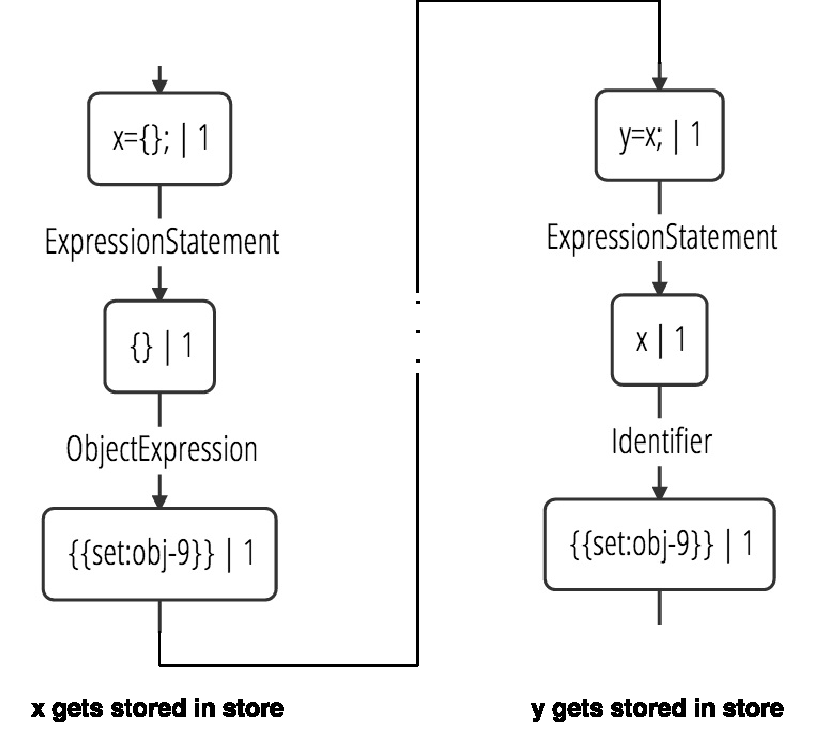
\includegraphics[width=.5\textwidth]{images/assignmentLookup} 
      \caption{Assignment representation in the state graph}
    \label{fig:AssignmentLookup}
\end{figure}


The problem with this kind of representation in the graph is that when we try to match the assignment in a query, no address information for \texttt{x} is available. After evaluating the fresh object, \texttt{x} gets stored in the store. Later on in the program, \texttt{y} gets assigned the value of \texttt{x}. Now, there is no problem because the address of \texttt{x} is already available in the store, so it can be looked up in the query. Note that the data flow detection in JS-QL is not as powerful as for example in a taint analysis. Queryies and policies can be written to mimic a taint-analysis, but this requires some work. Later in this chapter we will discuss how custom queries and policies can be defined.
\end{exmp}

\subsection{Negation}

Expressing which statements and expressions we want to detect on a path in the graph is made easy by JS-QL. Sometimes however, this does not suffice for some queries. For example, in some languages, accessing a file after it was closed results in an error in the application. This might compromise the integrity of the system. A naive approach to writing a policy for this would be to detect all calls to the \texttt{access} method that follow, after some wildcard states, the call of a \texttt{close} method for a file \texttt{f}. While this query would match and return all violations against the policy, false positives would occur. This is because of the wildcard states between the two function calls. One of these calls could be a call to the \texttt{open} method, meaning that accessing the file afterwards is permitted.  

\subsubsection*{Not: the language construct for negation}

A better approach would be to specify that we do \textit{not} want to encounter a call to \texttt{open} for \texttt{f} between closing and accessing it. This is exactly what the JS-QL \texttt{not} language construct does. When placing this construct right before a state, the query will only be matched if the negated state can not be matched with the current state in the state graph. When placing \texttt{not} before a state, and \texttt{star} or \texttt{plus} right after that state, it can be read as: ``Match zero/one or more states that are \textit{not} the negated state''. A better query for the example above would then be written as in listing \ref{lst:OpenClosedFile}, which can be found in the appendix for brevity reasons. The query first skips several states until it reaches a call to \texttt{close} on file \texttt{f}. The address of the file to be closed is also stored in a variable to correctly detect only the accessing and opening of that specific file. Next, all states are matched that are not opening \texttt{f}. Finally, the actual violation is detected, namely accessing the file after it has been closed and not re-opened. 

\subsubsection*{Limitations}

Negation is in the current version of JS-QL subject to some limitations: 
\begin{enumerate}
\item Variables that are bound in a negated state, are only visible to that state. They will thus not be included in the resulting substitutions.
\item Currently, only one state can be negated. Negating sequences of states wrapped in braces is not yet supported. We plan to resolve this in the future.
\end{enumerate}


\section{Types of queries}
\label{sec:TypesOfQueries}

The most straightforward way to query for properties is by just specifying a pattern and an input program. The pattern is then checked and each violating path is reported in the results. Sometimes however other types of queries are needed for the detection of specific policy violations. In this section we discuss the different types of queries and how they can be used.

\subsection{Existential queries}
Existential queries match a pattern \textit{if there exists a path} in the state graph matching the query. All queries presented so far are existential queries. They report a violation of a policy for each path on which they encounter the violation. Existential queries can be defined as follows:
\begin{definition}
\label{def:Existential}
\textbf{Existential queries}: Given an edge-labeled directed graph $G$ where labels may have parameters, a vertex $v_0$ in $G$, and a parametric regular-expression pattern $P$, compute all pairs of vertex $v$ in $G$ and a substitution $\theta$ for parameters in $P$ such that there exists a path from $v_0$ to $v$ in $G$ that matches some sentence accepted by $P$ under $\theta$.
\end{definition}

\noindent A consequence of definition \ref{def:Existential} is that \textit{any} path in the state graph matching user-defined query will produce a resulting substitution. For that path, the policy has been violated, but chances are that that path never gets executed when actually running the program, as a consequence of the overapproximations of the static analysis in JIPDA. A branch of a conditional might never be executed in a program for example. If the value of the test in the conditional gets overapproximated (i.e. with an abstract value of \textit{\{Bool\}}), the state graph will depict both branches, as it can't decide which branch will be taken. 

\subsection{Universal queries}

Universal queries provide stronger guarantees than existential queries, as they require that the query matches for the same substitutions along all possible paths in the state graph between two states. We define universal queries as follows:

\begin{definition}
\textbf{Universal queries}: Given an edge-labeled directed graph $G$ where labels may have parameters, a vertex $v_0$ in $G$, and a parametric regular-expression pattern $P$, compute all pairs of vertex $v$ in $G$ and substitution $\theta$ for parameters in $P$ such that every path from $v_0$ to $v$ in $G$ matches some sentence accepted by $P$ under $\theta$.
\end{definition}

The intrinsic difference between universal and existential queries is how they match a pattern. Where it suffices for existential queries that just one path exists in the state graph, universal queries make sure that \textit{all} paths between two points in the graph match the specified query. Example \ref{ex:Universal} shows an universal query:

\begin{exmp}
\label{ex:Universal}
Imagine a JS-QL predicate \texttt{def(\{name:'?x'\})}, which checks all definitions and redefinitions of a variable bound to \texttt{?x}. This variable has a constant value in the state graph as long as no redefinitions of \texttt{?x} happens along any path between two states in the graph. We can then query for each state in the graph where \texttt{?x} has a constant value. The query in listing \ref{lst:UniversalQuery} shows how this can be expressed in JS-QL. Creating such predicates will be discussed in the next section. The definition of a variable \texttt{v} is matched, and any state following that matched state that isn't a redefinition of \texttt{v} will be contained in the result. All states in the state graph up until a redefinition of \texttt{v} (or the end of the graph) will then be contained in the resulting substitution set.

\begin{lstlisting}[label={lst:UniversalQuery},language=JSQL, caption=Checking for constant folding using a universal query,mathescape=true]
G.skipZeroOrMore()
.def({name: '?x'})            // Define the variable
.not().def({name: '?x'}).star // As long as it isn't redefined
\end{lstlisting}

\end{exmp}

\subsection{Query direction}

In most traditional systems, queries are viewed as straightforward, in the sense that they match a part of a graph or other program representation from point $a$ to $b$. This way of reasoning implies that queries are always matched from the beginning to the end of a program (if control-flow information is available). 

Our tool supports this manner of querying in the traditional way, but also allows to explore the state graph bottom-up. This can be meaningful to search for certain program properties. Queries can explore the state graph in two ways:
\begin{enumerate}
\item \textit{Forward} queries are queries as we have defined them until now. They match the state graph from the beginning state to the final states of the state graph and are pretty easy to understand and read. 
\item \textit{Backward} queries on the other hand traverse the graph in a bottom-up manner, meaning that the query starts at the end of the state graph and matches states until the starting state of the graph is reached. 
\end{enumerate}

 Although backward queries are less common, they can be useful to perform some program analyses, such as live variables analysis. This analysis calculates for each program point the variables that may be potentially read before their next write. A variable is thus live if it holds a value that may be needed in the future. Example \ref{ex:Live} shows the backward query to perform a live analysis in JS-QL.

 \begin{exmp}
 \label{ex:Live}

 The \texttt{use} and \texttt{def} predicates in listing \ref{lst:Liveness} are again user-defined predicates. Starting from the resultstate of the program, some states are skipped until the first use of variable \texttt{?x} is found. Note that this is in fact the \textit{last} use of that variable in the state graph for that liveness set. The query then marks all states that aren't a write to \texttt{?x}. In this way, one or more states will be marked, representing the path on which variable \texttt{?x} was live.
\begin{lstlisting}[label={lst:Liveness},language=JSQL, caption=Live variables anlysis in JS-QL,mathescape=true]
G.skipZeroOrMore()
.use({name: '?x'})            // Read the variable 
.not().def({name: '?x'}).star // As long as it isn't written
\end{lstlisting}
\end{exmp}

\section{Defining predicates and policies}
\label{sec:DefiningPolicies}


Expressing vulnerabilities with only the \texttt{state} and \texttt{wildcard} constructs quickly becomes tiresome as every attribute of the state has to be explicitly specified. Our tool remedies this by letting users specify their own predicates and policies as well by providing some basic customizable predicates for single expressions and statements.
We can distinguish predicates and policies by what they match. 
\begin{enumerate}
\item \textit{Predicates} are like the \texttt{state} construct, in the sense that they match only one specific state. For example, JS-QL has a built-in predicate \texttt{functionCall} which matches function calls. Predicates are useful in the sense that a user can specify what he wants to match in a state.
\item \textit{Policies} on the other hand are sequences of predicates and/or \texttt{state}s, forming a query pattern. 
\end{enumerate}

\subsection{Creating a predicate}

This section demonstrates how to write predicates by dissecting a relatively simple built-in predicate called \texttt{assign}. The full code for the predicate is listed in listing \ref{lst:assignPredicate} in the appendix.

\subsubsection*{Signature of a predicate}
All predicates and policies can be written in a separate file, as long as they are extend in the \textit{JSQL prototype}:\\
\texttt{JSQL.prototype.assign = function(obj)\{\ldots \}}\\
This is the basic notation for named predicates, in this case the \texttt{assign} predicate. The dots in the code above will be filled in by the actual predicate code. The \texttt{obj} argument represents the map of all properties of the state that need to be matched. The user is free in which properties and attributes he wishes to match or omit for a specific query, as discussed in the next section.

\subsubsection*{Specifying what a predicate has to match} 

The usefulness of predicates would drastically be reduced if the user has to again pass a nested map of properties to the predicate. We therefore let the developer of the predicate decide which properties he wishes to match, and how he names these properties in the predicate. We illustrate this in example \ref{ex:Attributes}.

\begin{exmp}
\label{ex:Attributes}
For the \texttt{assign} predicate, 3 basic attributes can be specified in the \texttt{obj} argument: \texttt{this}, \texttt{left} and \texttt{right}, representing the whole assignment node, its left- and right-hand side resp. In the definition of the predicate, a user can specify this as in listing \ref{lst:predicateArguments}.

\begin{lstlisting}[label={lst:predicateArguments},language=JavaScript, caption=State properties of the \texttt{assign} predicate,mathescape=true]
var s = {}; // variable representing the state
var objThis  = this.getTmpIfUndefined(obj.this);  //optional
var objLeft  = this.getTmpIfUndefined(obj.left);  //optional
var objRight = this.getTmpIfUndefined(obj.right); //optional
//The following would make the right attribute mandatory 
var objRight = obj.right;                         //mandatory
\end{lstlisting}

Variable \texttt{s} will contain all information that we wish to match agains a state in the state graph.
When accessing a key in the \texttt{obj} map (like \texttt{obj.left}), the corresponding value is returned when found. When no such key exists, JavaScript returns \texttt{undefined}. To ease the use of predicates, some attributes in the \texttt{obj} map can be made optional. This is done by using the \texttt{getTmpIfUndefined} method, which returns a \textit{temporary variable} when the value for its argument is \texttt{undefined}, and the regular value (a literal or a variable) when it is contained in the map. 
\end{exmp}

\subsubsection*{Temporary variables}

 Temporary variables are variables that won't be contained in the resulting substitutions. By introducing these variables in the code, no conditionals have to be written that check whether an attribute has been specified in the \texttt{obj} map when a predicate is used, as we can just use a temporary variable as a replacement. In this way, a predicate also provides information that can be queried optionally.

%nieuwe sectie
\subsubsection*{Mapping attributes to the state graph}

The \textit{state chain} of a pattern state represents all information that has to be matched against the state graph.
The state chain can be set up by mapping the attributes of the \texttt{obj} to a state in the state graph. To make things not too complicated for query and predicate developers, we provide a \texttt{setupStateChain} method which does just that. The \texttt{s} variable from example \ref{ex:Attributes} will be used to build the pattern state corresponding to a state the state graph. For each attribute that we provide through the predicate, an entry has to be made in \texttt{s}. This is illustrated in example \ref{ex:StateChain}.

\begin{exmp}
\label{ex:StateChain}
 As seen in listing \ref{lst:predicateState}, \texttt{setupStateChain} takes three arguments:
 \begin{enumerate}
 \item The first argument represents the pattern state that is set up throughout the predicate. \texttt{setupStateChain} will add one attribute to the pattern state, depending on its second argument.
 \item The second argument specifies the nested map that needs to be matched in the state graph. This argument is an array of keys that has to be read from left to right. Each entry goes one level deeper in the nested map, starting from the first entry of the array, which is a JS-QL keyword. The last entry of the array is the key whose corresponding value will be matched with the third argument of \texttt{setupStateChain}.
 \item The third argument represents the literal or variable that needs to be matched against the last element of the second argument. This argument corresponds with either a variable previously defined, as in example \ref{ex:Attributes}, or a literal, as can be seen on line 4 of the example code.
 \end{enumerate}

Note that \texttt{setupStateChain} is not limited to querying the \texttt{node} property of a state. All information in the state graph can be queried through a predicate.

\begin{lstlisting}[label={lst:predicateState},language=JavaScript, caption=State chain setup of the \texttt{assign} predicate,mathescape=true]
this.setupStateChain(s,['node','this'], objThis);
this.setupStateChain(s,['node','expression','left'], objLeft);
this.setupStateChain(s,['node','expression','right'], objRight); 
this.setupStateChain(s,['node','expression','operator'], '='');
\end{lstlisting}
\end{exmp}

%nieuwe sectie
\subsubsection*{Additional predicate information}
 JS-QL allows to specify properties, filters and lookups for predicates in the same way as for states. Putting everything together happens by finalizing each predicate state (only \texttt{s} in this case) and specifying the state(s) that match the predicate/policy. Example \ref{ex:predicateFinalize} shows how finalization is done and how the pattern is specified. 


 Finalizing handles lookups, filters and properties through the \texttt{finalize} method. This method extracts all relevant information from the \texttt{obj} map and adds it to the pattern state, which it receives as a first argument. Finally, the full predicate or policy pattern is specified and each state in the pattern or pattern gets initialized with its own designated pattern state. For predicates, there will always be at most one pattern state. Policies however can have multiple pattern states, as they represent a sequence of states, each with their own pattern state. This is the only characteristic in which predicates and policies differ. An example of a policy can be seen in listing \ref{lst:WriteToBuiltinObjectPrototype} in the appendix.

\begin{exmp}
\label{ex:predicateFinalize}
Defining a predicate always ends with the finalization of the pattern state. When finalized, the state map is passed to the \texttt{state} language construct, containing all information that has to be queried by the predicate.
\begin{lstlisting}[label={lst:predicateFinalize},language=JavaScript, caption=Finalizing the \texttt{assign} predicate,mathescape=true]
this.finalize(s, obj); //Finalize a specific state
return this.state(s);  //Fill in pattern state s
\end{lstlisting}

\end{exmp}

We can now use this predicate in any query, with the arguments that we wish to match in a state, as seen in Listing \ref{lst:assignCall}:

\begin{lstlisting}[label={lst:assignCall},language=JSQL, caption=Using the \texttt{assign} predicate,mathescape=true]
G.skipZeroOrMore().assign({left: '?l', right: '?r'})
G.skipZeroOrMore().assign({right: '?r', this: '?t', left: '?l'})
G.skipZeroOrMore().assign({left: '?l', right:'?r',
                           properties:{
                              '?rName' : '?r.name'
                           },
                           lookup:{
                              '?rName' : '?rAddr'
                           }}) 
//...
\end{lstlisting}

\subsection{Recursion}
%moet dit naar types of queries?
 Recursive queries are queries that can invoke themselves again, until a base case is matched. This type of query can for example be used to detect by which variables a variable is tainted (i.e. influenced/marked). JS-QL supports recursive queries by providing the \texttt{rec} function. This function takes two arguments: 
\begin{enumerate}
\item The first argument represents the mapping for the next recursive step.
\item The second argument is the policy or predicate that has to be called recursively.
\end{enumerate}

 The \texttt{taintedBy} policy is included in the appendix as listing \ref{lst:taintedBy}. It describes a naive taint analysis which only considers simple assignments. It takes three arguments, which can all be omitted: \texttt{orig} denotes the original value which will be aliased, \texttt{alias} represents the alias of the original value and \texttt{rec} keeps track of all variables that have been used as aliases inbetween \texttt{orig} and \texttt{alias}. The relevant code of the policy is found in example \ref{ex:Recursion}:

\begin{exmp}
\label{ex:Recursion}
The policy matches all simple assignments by name. Lines 1-8 set up the state maps of 2 separate states. The first state matches a direct assignment from \texttt{orig} to \texttt{alias}. The second state does the same, but the alias in this case is an intermediate assigned variable \texttt{flow}. When $a$ is assigned to $b$ and $b$ to $c$, the resulting state looks like: \{orig: a, flow: b, alias: c\}, indicating that $c$ is an alias of $a$, and that it obtained the value of $a$ through $b$. Lines 10-16 show the pattern that needs to be matched. 

We either match an assignment directly (the base case), or we match a state from \texttt{orig} to \texttt{flow}, and later in the graph from \texttt{flow} to \texttt{alias}. The recursive call will keep occuring until no more match is found in the state graph, or when the base case is matched. This policy shows that recursive queries can also be used to discover data flow properties of a program.

\begin{lstlisting}[label={lst:recursivePolicy},language=JSQL, caption=Recursive call of the \texttt{taintedBy} policy,mathescape=true]
this.setupStateChain(s1, //State map s1
                    ['node','expression','right','name'], orig); 
this.setupStateChain(s1, //State map s1
                    ['node','expression','left','name'], alias); 
this.setupStateChain(s2, //State map s2
                    ['node','expression','right','name'], orig);
this.setupStateChain(s2, //State map s2
                    ['node','expression','left','name'], flow);

return this .lBrace()
            .state(s1)                  //1. From orig to alias
            .or()
            .state(s2)                  //2. From orig to flow
            .skipZeroOrMore()           //   Skip some states
            .rec(newObj,this.taintedBy) //   From flow to alias
            .rBrace();

//JS-QL query:
G.skipZeroOrMore({orig: '?o', alias:'?alias', rec:'?r'})
\end{lstlisting}

\end{exmp}

\section{Conclusion}
In this chapter we presented the JS-QL language. We described the syntax and semantics of its language constructs. We first explained how the basic state construct can be used to match the state graph. Wildcards in JS-QL enable users to specify that some states in the state graph can be skipped. Next, we described how to express disjunction in queries to allow for multiple matching paths in a single query. Additional properties and filters can also be specified in JS-QL, as well as the lookup of addresses and values of variables and functions. Finally, the JS-QL language construct for negation enables to specify the negation of basic states. This can be used to ensure that a state does not occur on the matched path.

We described the two types of queries that JS-QL supports. Existential queries match a pattern if at least one path is found, whereas universal queries require that the query matches for the same substitutions along all possible paths in the state graph between two states. Both types of queries can be used to explore the state graph. This exploration can be done traditionally by using forward queries, or by using backward queries to detect other program properties.

 Finally, we discussed the difference between predicates and policies, and described how users can create pthem. Recursion in predicates and policies is also supported by JS-QL, as these kind of queries are useful for certain program analysis queries.




